\documentclass{article}
\usepackage{amsmath}
\usepackage{amssymb}
\usepackage{algorithm}
\usepackage{float}
\usepackage{color}
\usepackage{multicol}
\usepackage{forloop}
\usepackage{graphicx}
\usepackage[margin=0.8in]{geometry}
\usepackage{caption}
\usepackage{enumerate}
\usepackage{systeme}
\graphicspath{ {.} }
\title{STAT 2509B4 \\
	\large{Assignment 4}}
\author{Krystian Wojcicki, 101001444}
\date{Winter 2020}

\begin{document}
\maketitle

\begin{enumerate}[1.]

\item \textbf{ Christmas week is a critical period for most ski resorts. Because many students and
adults are free, they are able to spend several days indulging in their favorite pastime,
skiing. A ski resort in Vermont wanted to determine the effect that weather had on their
sales of lift tickets. The manager of the resort collected the number of lift tickets sold
during the Christmas week (y), the total snowfall ($x_1$) and the average temperature ($x_2$)
for the past 20 years ($x_3$). The TSS for the full model
$y = \beta_0 + \beta_1x_1 + \beta_2x_2 + \beta_3 x_3 + \epsilon$ is : TSS $= 56 601 012$
We decided to screen the independent variables to determine the best set for predicting the lift
tickets sales. The sums of squares for all possible regression models were found to be as
follows: 
\begin{center}
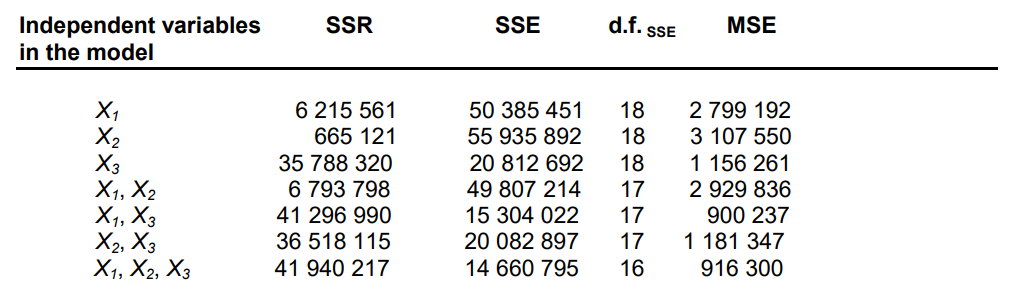
\includegraphics[scale=0.5]{a4_q1}
\end{center}}

\begin{enumerate}[(a)]
\item \textbf{Determine the subset of variables that is selected as best by the Forward Selection Procedure using $F_0^* = 4.2$ (to-add-variable). Show your steps. }

\begin{enumerate}[(1)]
\item Fit all one term models: $y = \beta_0 + \beta_1x_j + \epsilon$ for $j = 1,2,3$ \\
SSR$(X_1) = 6 215 561$ \\
SSR$(X_2) = 665 121$ \\
SSR$(X_3) = 35 788 320 \Rightarrow $ max \\

Therefore $F_3 = \frac{\text{MSR}(X_3)}{\text{MSE}(X_3)} = \frac{\text{SSR}(X_3)/1}{\text{SSE}(X_3)/18} = \frac{35 788 320/1}{20 812 692/18} = 30.952$

Since $F_3 = 30.952 > F_0 = 4.2$ we keep $X_3$

\item Fit all two term models $y = \beta_0 + \beta_1x_3 + \beta_2x_j + \epsilon$ for $j = 1,2$ \\

Calculate SSR$(X_j | X_3)$ \\

SSR$(X_1 | X_3) = \text{SSR}(X_1, X_3) - \text{SSR}(X_3) = 41 296 990 - 35 788 320 = 5 508 670 \Rightarrow$ max\\ 
SSR$(X_2 | X_3) = \text{SSR}(X_2, X_3) - \text{SSR}(X_3) = 36 518 115 - 35 788 320 = 729 795$

Therefore $F_1 = \frac{  \text{MSR}(X_1 | X_3) }{  \text{MSE}(X_1, X_3) } = 
\frac{ [ \text{SSR}(X_1, X_3) - \text{SSR}(X_3) ] / [ df_{SSR(X_1, X_3)} - df_{SSR(X_3)} ]
}{
\text{SSE}(X_1, X_3) / df_{SSE(X_1, X_3)}
}
=  \frac{
 5 508 670 / (2- 1)
}{
15 304 022 / 17
} = 6.1191358716$

Since $F_1 = 6.1191358716 > 4.2$ we keep $X_1, X_3$

\item Fit the full model $y = \beta_0 + \beta_1x_3 + \beta_2x_1 + \beta_3x_3 + \epsilon$

Calculate SSR$(X_2 | X_1, X_3) = \text{SSR}(X_1, X_2, X_3) - \text{SSR}(X_1, X_3) = 41 940 217  - 41 296 990 = 643227$

Therefore $F_2 = \frac{  \text{MSR}(X_2 | X_1, X_3) }{  \text{MSE}(X_1, X_2, X_3) } = 
\frac{ [ \text{SSR}(X_1,X_2, X_3) - \text{SSR}(X_1, X_3) ] / [ df_{SSR(X_1,X_2, X_3)} - df_{SSR(X_1, X_3)} ]
}{
\text{SSE}(X_1,X_2, X_3) / df_{SSE(X_1, X_2, X_3)}
}
=  \frac{
643 227 / (3 - 2)
}{
14 660 795 / 16
} = 0.701983214416$

Since $F_2 \leq F_0^*$ we keept $X_1, X_3$

\end{enumerate}

Therefore the best set is $\{X_1, X_3\}$

\item \textbf{Determine the subset of variables that is selected as best by the Backward Elimination
Procedure using $F_0^{**} = 4.1$ (to-delete-variable). Show your steps.
NOTE: $( t_0^{**} )^2 = F_0^{**}$}

Fit the full model $y = \beta_0 + \beta_1x_1 + \beta_2x_2 + \beta_3 x_3 + \epsilon$ and check whether model is significant or not at $\alpha=5\%$.

$F = \frac{\text{MSR}_f}{\text{MSE}_f} = \frac{\text{SSR}_f / 3}{\text{SSE}_f / 16} = \frac{ 41 940 217/3}{14 660 795/16} = 15.2570960397$

Since $F = 15.2570960397 > F_{(3, 16); 0.05} = 3.24$, we can conclude that at 5\% level of sigificance the full model is significant and can be used

\begin{enumerate}[(1)]

\item Calculate $F_j = (t_j)^2 = \frac{ \text{MSR}(X_j | \text{all} X \text{'s except} X_j) }{\text{MSE}(X_1, X_2, X_3)} = \frac{ [SSR_f - SSR(\text{all} X\text{'s except} X_j)]/df}{MSE_f}$ for $j = 1,2,3$

$F_1 =
\frac{ MSR(X_1 | X_2, X_3)
}{
MSE(X_1, X_2, X_3)
}
=
\frac{
[SSR(X_1, X_2, X_3) - SSR(X_2, X_3)]/[df_{SSR(X_1,X_2,X_3)} - df_{SSR(X_2,X_3)}]
}{
SSE(X_1, X_2, X_3)/df_{SSE(X_1, X_2, X_3)}
}
= 
\frac{
[41 940 217 - 36 518 115]/[3 - 2]
}{
14 660 795 / 16
}
= 5.91738933666
$

$F_2 =
\frac{ MSR(X_2 | X_1, X_3)
}{
MSE(X_1, X_2, X_3)
}
=
\frac{
[SSR(X_1, X_2, X_3) - SSR(X_1, X_3)]/[df_{SSR(X_1,X_2,X_3)} - df_{SSR(X_1,X_3)}]
}{
SSE(X_1, X_2, X_3)/df_{SSE(X_1, X_2, X_3)}
}
= 
\frac{
[41 940 217 - 41 296 990]/[3 - 2]
}{
14 660 795 / 16
}
= 0.701983214416 \Leftarrow \text{min}
$

$F_3 =
\frac{ MSR(X_3 | X_1, X_2)
}{
MSE(X_1, X_2, X_3)
}
=
\frac{
[SSR(X_1, X_2, X_3) - SSR(X_1, X_2)]/[df_{SSR(X_1,X_2,X_3)} - df_{SSR(X_1,X_2)}]
}{
SSE(X_1, X_2, X_3)/df_{SSE(X_1, X_2, X_3)}
}
= 
\frac{
[41 940 217 - 6 793 798]/[3 - 2]
}{
14 660 795 / 16
}
= 38.3569038378
$

Since $F_2 \ngtr 4.1$ we remove $x_2$ from the model.

\item Fit model $y = \beta_0 + \beta_1x_1 + \beta_3x_3 + \epsilon$

$F_1 =
\frac{ MSR(X_1 | X_3)
}{
MSE(X_1, X_3)
}
=
\frac{
SSR(X_1, X_3) - SSR(X_3)
}{
SSE(X_1,X_3)/df_{SSE(X_1, X_3)}
}
= 
\frac{
(41 296 990 - 35 788 320)
}{
(15 304 022 / 17)
}
= 6.1191 \Leftarrow \text{min}
$

$F_3 =
\frac{ MSR(X_3 | X_1)
}{
MSE(X_1, X_3)
}
=
\frac{
SSR(X_1, X_3) - SSR(X_1)
}{
SSE(X_1,  X_3)/df_{SSE(X_1, X_3)}
}
= 
\frac{
(41 296 990 - 6 215 561 )
}{
(15 304 022 / 17)
}
= 38.9691215159
$

Since $F_1 = 6.1191 > 4.1$ we remove nothing and keep the current model as the final model and terminate the procedure.

Therefore the best set is $\{X_1, X_3\}$.

\end{enumerate}

\item \textbf{Determine the subset of variables that is selected as best by the Stepwise Regression
Procedure using $F_0^* = 4.2$ (to-add) and $F_0^{**} = 4.1$ (to-delete). Show your steps. }

\begin{enumerate}[(1)]
\item Fit all one term models: $y= \beta_0 + \beta_1x_j + \epsilon$ for $j = 1,2,3$
As we saw in forward selection in part (a) we know that we keep $X_3$

\item Fit all two term models $y = \beta_0 + \beta_1x_3 + \beta_2x_j + \epsilon$ for $j = 1,2$
As we saw in forward selection in part (a) we know that we keep $X_1$ \\

Now check if after adding $X_1$, $X_3$ became insignificant. 

$F_3 = \frac{ SSR(X_3 | X_1) }{ MSE(X_1, X_3)} = \frac{ SSR(X_1, X_3) - SSR(X_1)}{SSE(X_1, X_3)/df_{SSE(X_1, X_3)}} = \frac{41 296 990 - 6 215 561}{15 304 022/ 17} = 38.9691215159$

Since $F_3 = 38.9691215159 > F_0^{**} = 4.1$ we keep  $X_3$ and keep $X_1$. 

\item Fit the full model: $y = \beta_0 + \beta_1x_3 + \beta_2x_1 + \beta_3x_2 + \epsilon$
As we saw in forward selection in part (a) we know that we dont not add $X_2$ and there is no need to check if adding $X_2$ makes any variable redundant. Therefore the best set is ${X_1, X_3}$.

\end{enumerate}

\end{enumerate}

\item \textbf{A quality engineer in a company manufacturing electronic audio equipment was inspecting
 a new type of battery that was being considered for use. A batch of 20 batteries was
 randomly assigned to four groups (so that there were five batteries per group). Each group
 of batteries was then subjected to a particular pressure level – low, normal, high, very
 high. The batteries were simultaneously tested under these pressure levels and the times
 to failure (in hours) were recorded and are given below:
\begin{center}
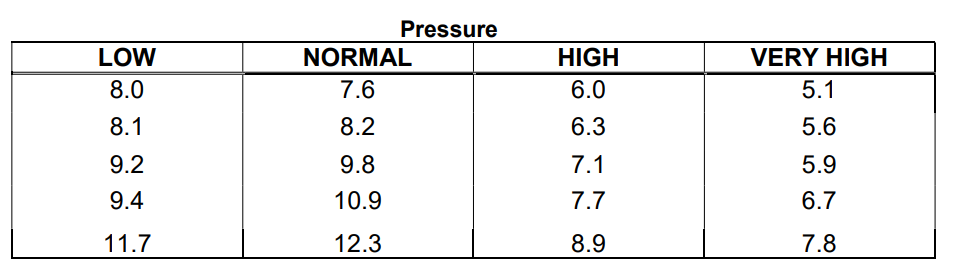
\includegraphics[scale=0.5]{a4_q2}
\end{center}
Establish whether the average times to battery failure are the same for the four pressure levels;
if not, do a follow-up analysis to determine which are the same and which differ. (Use $\alpha =0.10$).
List all necessary assumptions and indicate which might be suspect. Also perform a nonparametric analysis. Verify your results using SAS. }

C.R.D
Assume 
\begin{enumerate}[1)]
\item 3 independent random samples of patients (given) TODO
\item 3 normally distributed patient groups
\item with equal variance, $\sigma^2$ (potentially)
\end{enumerate}

To check the assumption of equal variance using Hartleys test we need $s_i^2$'s for $j = 1,2,3, 4$ where $n_1 = n_2 = n_3 = n_4 = 5, k = 4, \bar{n} = 5, [\bar{n}] = 5, n = 20$

$s_1^2 = \frac{
\sum_{j=1}^{n_1} {y_{1j}^2} - \frac{ (\sum_{j=1}^{n_1}{y_{1j}})^2}{n_1}
}{
n_1 - 1
}
=
\frac{
439.5 - 46.4^2 / 5
}{4}
= 2.227
$


$s_2^2 = \frac{
\sum_{j=1}^{n_2} {y_{2j}^2} - \frac{ (\sum_{j=1}^{n_2}{y_{2j}})^2}{n_2}
}{
n_2 - 1
}
=
\frac{
491.14 - 48.8^2 / 5
}{4}
= 3.713 \Leftarrow \text{max}
$

$s_3^2 = \frac{
\sum_{j=1}^{n_3} {y_{3j}^2} - \frac{ (\sum_{j=1}^{n_3}{y_{3j}})^2}{n_3}
}{
n_3 - 1
}
=
\frac{
264.6 - 36^2 / 5
}{4}
= 1.35
$


$s_4^2 = \frac{
\sum_{j=1}^{n_4} {y_{4j}^2} - \frac{ (\sum_{j=1}^{n_4}{y_{4j}})^2}{n_4}
}{
n_4 - 1
}
=
\frac{
197.91 - 31.1^2 / 5
}{4}
= 1.117 \Leftarrow \text{min}
$ \\


$H_0: \sigma_1^2 = \sigma_2^2 = \sigma_3^2 = \sigma_4^2$ \\
$H_a:$ atleast one of the $\sigma^2$'s $\neq $\\
$ \alpha = 0.01$ or 0.05

Test statistic $F_{max} = \frac{s_{max}^2}{s_{min}^2} = 3.713 / 1.117 = 3.324$

Rejection Region we reject $H_0$ if $F_{max} > F_{max(k, [\bar{n}]-1); \alpha} =
\syslineskipcoeff{1}
\systeme*{F_{max(4, 4);0.01}=49,F_{max(4,4);0.05} = 20.6}
$

Since 3.324 is not greater than 20.6 (or 49) we can conclude that at a 1\% (or 5\%) level of significance there is no evidence to say that the variances are not equal (i.e we have equal variance). Therefore we may proceed with the main test

$G.T. = \sum_{i=1}^{k}{ \sum_{j=1}^{n_i}{y_{ij}}} = \sum_{i=1}^{k}{T_i} = 162.3$ \\
$TSS = \sum_{i=1}^{k}{ \sum_{j=1}^{n_i}{y_{ij}^2}} - \frac{(G.T)^2}{n} = 1393.15 - \frac{162.3^2}{20} = 76.0855$ \\
$SST_r = \sum_{i=1}^{k}{ \frac{T_i^2}{n_i}} - \frac{(G.T)^2}{n}  = [(46.4)^2/5 + (48.8)^2/5 + (36^2)/5 + (31.1)^2/5] - \frac{162.3^2}{20} = 42.4575$ \\
$SSE = TSS - SST_r = 76.0855 - 42.4575 = 33.628$\\
$MST_r = \frac{SST_r}{k - 1} = 42.4575 / 3 = 14.1525$ \\
$MSE = \frac{SSE}{n - k} = 33.628/16 = 2.10175$ \\
$F_T = \frac{MST_r}{MSE} = 14.1525/2.10175 = 6.73367431902 = 6.733$ \\


\begin{center}
 \begin{tabular}{||c c c c c||} 
 \hline
Source & d.f & SS & MS & F \\ [0.5ex] 
 \hline\hline
Regression & 3 & 42.4575 & 14.1525 & 6.733 \\
 \hline
Error & 16 & 33.628 & 2.10175 &  \\
 \hline
Total & 19  &  76.0855 & & \\ [1ex]
 \hline
\end{tabular}
\end{center}

$H_0: \mu_1 = \mu_2 = \mu_3 = \mu_4$ \\
$H_a:$ at least one of the $\mu's \neq$ \\
$\alpha = 0.10$

Test statistic $F_T = \frac{MST_r}{MSE} = 6.733$

Rejection Region: we reject $H_0$ if $F_T > F_{(k-1, n-k);\alpha} = F_{(3, 16);0.10} = 2.460$

Since $F_T = 6.733 > 2.460$ we reject $H_0$ and conclude that at a 10\% level of significance there is evidence to say the time to battery failure is different among the four different pressure levels.

Which are different: Use Tukey's h.s.d

\begin{enumerate}[1)]

\item $k \choose 2 $ = $4 \choose 2$ $= 6$ pairs of $|\bar{y_i} - \bar{y_j}|$ \\
$H_0: \mu_i = \mu_j$ \\
$H_a: \mu_i \neq \mu_j$ \\
for i,j = 1,2,3,4 and i $\neq$ j

\item h.s.d $ = q_{\alpha(k ,v)} \times \sqrt{ \frac{MSE}{2}( \frac{1}{n_i} + \frac{1}{n_j}) } = q_{0.10(4, 16)} \times \sqrt{ \frac{2.10175}{2}\frac{2}{5}} = (3.52003)(0.64834404447) = 2.28219048686 = 2.282 $

$\bar{y_1} = \frac{T_1}{n_1} = 46.4/5 = 9.28$\\
$\bar{y_2} = \frac{T_2}{n_2} = 48.8/5 = 9.76$\\
$\bar{y_3} = \frac{T_3}{n_3} = 36/5 = 7.2$\\
$\bar{y_4} = \frac{T_4}{n_4} = 31.1/5 = 6.22$\\

\item $| \bar{y_1} - \bar{y_2} | = 0.48 < 2.282 \Rightarrow \mu_1 = \mu_2$ \\
$| \bar{y_1} - \bar{y_3} | = 2.08 < 2.282 \Rightarrow \mu_1 = \mu_3$ \\
$| \bar{y_1} - \bar{y_4} | = 3.06 > 2.282 \Rightarrow \mu_1 \neq \mu_4$ \\
$| \bar{y_2} - \bar{y_3} | = 2.56 > 2.282 \Rightarrow \mu_2 \neq \mu_3$ \\
$| \bar{y_2} - \bar{y_4} | = 3.54 > 2.282 \Rightarrow \mu_2 \neq \mu_4$ \\
$| \bar{y_3} - \bar{y_4} | = 0.98 < 2.282 \Rightarrow \mu_3 = \mu_4$ \\

Therefore there are differences in average time for battery failure for (low and very high), (normal and high), (normal and very high) groups.

\end{enumerate}

None-parametric Analysis (Kruskal-Wallis test)
Assume:
\begin{enumerate}[1)]
\item C.R.D (4 independent random samples from 4 treatment populations) with
\item approximately the same shape and spread
\end{enumerate}

First we need to rank the observations from smallest to the largest


\begin{center}
 \begin{tabular}{||c c c c||} 
 \hline
Low & Normal & High & Very High \\ [0.5ex] 
 \hline\hline
8.0 (11) & 7.6 (8) & 6.0 (4) & 5.1 (1) \\
 \hline
8.1 (12) & 8.2 (13) & 6.3 (5) & 5.6 (2) \\
 \hline
9.2 (15) & 9.8 (17) & 7.1 (7) & 5.9 (3) \\
 \hline
9.4 (16) & 10.9 (18) & 7.7 (9) & 6.7 (6) \\
 \hline
11.7  (19) & 12.3 (20) & 8.9 (14) & 7.8 (10) \\ [1ex]
 \hline
\end{tabular}
\end{center}

$T_{R_1} = 73, T_{R_2} = 76, T_{R_3} = 39, T_{R_4} = 22$

Check $\frac{n(n+1)}{2} = \frac{20\times21}{2} = 210$
$73 + 76 + 39 + 22 = 210$

$H_0: Md_1 = Md_2 = Md_3$ \\
$H_a$: at least one of the $Md$'s $\neq$. \\
$\alpha = 0.10$

$H = \frac{12}{n(n+1)}[\sum_{i=1}^{k}{ \frac{T_{R_i}^2}{n_i}}] - 3(n+1) = \frac{12}{20\times21}[\frac{73^2}{5} + \frac{76^2}{5} + \frac{39^2}{5} + \frac{22^2}{5} ] - 3(21) = 11.91$

Rejection region, we reject $H_0$ if $H > \chi_{(k-1);\alpha}^2 = \chi_{3; 0.10}^2 = 6.251$

Since $H = 11.91 > 6.251$ we reject $H_0$. and conclude that at a 10\% level of significance there is evidence to say that the medians vary among the 4 pressures.

Which pressures differ? Dunes procedure:

\begin{enumerate}[1)]
\item
Calculate $k \choose 2$ = $4 \choose 2$ = 6 pairs of $|\bar{R_i} - \bar{R_j}|$ for $H_0: Md_i = Md_j$ vs $H_a: Md_i \neq Md_j$ \\
for $i,j = 1,2,3,4$ and $i \neq j$

\item 
Critical range = $z_{\frac{\alpha}{k(k-1)}} \times \sqrt{ \frac{n(n+1)}{12}( \frac{1}{n_i} + \frac{1}{n_j} )} = z_{\frac{0.1}{4(3)}} \times \sqrt{ \frac{20(21)}{12}\frac{2}{5}} = 2.395(3.74) = 8.9573$

$\bar{R_1} = \frac{T_{R_1}}{n_1} = 73/5 = 14.6$ \\
$\bar{R_2} = \frac{T_{R_2}}{n_2} = 76/5 = 15.2$ \\
$\bar{R_3} = \frac{T_{R_3}}{n_3} = 39/5 = 7.8$ \\ 
$\bar{R_4} = \frac{T_{R_4}}{n_4} = 22/5 = 4.4$\\ 

\item
$|\bar{R_1} - \bar{R_2}| = 0.6 < 8.96 \Rightarrow Md_1 = MD_2$ \\
$|\bar{R_1} - \bar{R_3}| = 6.8 < 8.96 \Rightarrow Md_1 = MD_3$ \\
$|\bar{R_1} - \bar{R_4}| = 10.2 > 8.96 \Rightarrow Md_1 \neq MD_4$ \\

$|\bar{R_2} - \bar{R_3}| = 7.8 < 8.96 \Rightarrow Md_2 = MD_3$ \\
$|\bar{R_2} - \bar{R_4}| = 10.8 > 8.96 \Rightarrow Md_2 \neq MD_4$ \\

$|\bar{R_3} - \bar{R_4}| = 3.4 < 8.96 \Rightarrow Md_3 = MD_4$ \\

\end{enumerate}

Therefore there are differences in medians of battery failure for (low and very high), (normal and very high) groups.


\item \textbf{An experiment was conducted by a private research corporation to investigate the toxic
effects of three chemicals (I, II and III) used in the tire-manufacturing industry. In this
experiment 1-inch squares of skin on rats were treated with the chemicals and then scored
from 0 to 10, depending on the degree of irritation. Three adjacent 1-inch squares were
marked on the back of each of eight rats, and each of the three chemicals was applied to
each rat. The data are as shown in the table. 
\begin{center}
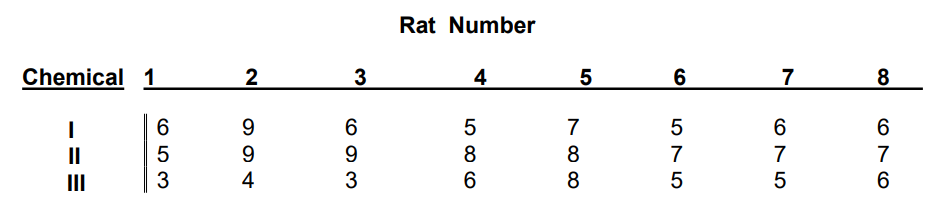
\includegraphics[scale=0.5]{a4_q3}
\end{center}
Is it possible to be $95\%$ certain that the toxic effects of three chemicals are not equal? Conduct
the appropriate follow-up analysis (use $\alpha = 0.05$) to establish which means are significantly
different. List all necessary assumptions and indicate which might be suspect. Also perform a
non-parametric analysis. Verify your results using SAS. }


R.B.D
Assume 
\begin{enumerate}[1)]
\item random samples of 3 different chemicals randomly assigned to 8 different rats (given)
\item populations corresponding to each chemical-rat combination are normally distributed
\item with equal variance, $\sigma^2$ (?)
\item no interactions between chemicals and rats
\end{enumerate}

To check the assumption of equal variance using Hartley's test we need $s_i^2$'s for $i = 1,2,3$ where $n_1 = n_2 = n_3 = 8, k = 3, b=8, \bar{n} = n = 8, [\bar{n}] = 8, n = 24$

$s_1^2 = \frac{
\sum_{j=1}^{b} {y_{1j}^2} - \frac{ (\sum_{j=1}^{b}{y_{1j}})^2}{b}
}{
b - 1
}
=
\frac{
324 - 50^2 / 8
}{7}
= 1.6428 \Leftarrow min
$

$s_2^2 = \frac{
\sum_{j=1}^{b} {y_{2j}^2} - \frac{ (\sum_{j=1}^{b}{y_{2j}})^2}{b}
}{
b - 1
}
=
\frac{
462 - 60^2 / 8
}{7}
= 1.71428571429
$

$s_3^2 = \frac{
\sum_{j=1}^{b} {y_{3j}^2} - \frac{ (\sum_{j=1}^{b}{y_{3j}})^2}{b}
}{
b - 1
}
=
\frac{
220 - 40^2 / 8
}{7}
= 2.85714285714 \Leftarrow max
$

$H_0: \sigma_1^2 = \sigma_2^2 = \sigma_3^2$ \\
$H_a:$ atleast one of the $\sigma^2$'s $\neq $\\
$ \alpha = 0.01$ or 0.05

Test statistic $F_{max} = \frac{s_{max}^2}{s_{min}^2} = 2.85714285714 / 1.6428 = 1.73919092838$

~~~~~~~~~~~~~
Rejection Region we reject $H_0$ if $F_{max} > F_{max(k, [\bar{n}]-1); \alpha} =
\syslineskipcoeff{1}
\systeme*{F_{max(4, 4);0.01}=15.980,F_{max(4,4);0.05} = 6.390}
$

Since 3.324 is not greater than 6.390 (or 15.980) we can conclude that at a 1\% (or 5\%) level of significance there is no evidence to say that the variances are not equal (i.e we have equal variance). Therefore we may proceed with the main test
~~~~~~~~~~
 TODO

$G.T. = \sum_{i=1}^{k}{ \sum_{j=1}^{b}{y_{ij}}} = \sum_{i=1}^{k}{T_i} = 150$ \\
$TSS = \sum_{i=1}^{k}{ \sum_{j=1}^{b}{y_{ij}^2}} - \frac{(G.T)^2}{bk} = 1006 - \frac{150^2}{24} = 68.5$ \\
$SST_r = \sum_{i=1}^{k}{ \frac{T_i^2}{b}} - \frac{(G.T)^2}{bk}  = [(50)^2/8 + (60)^2/8 + (40)^2/8] - \frac{150^2}{24} = 25$ \\
$SSB = \sum_{j=1}^{b}{ \frac{B_j^2}{k} - \frac{(G.T)^2}{bk}}  = [(14)^2/3 + (22)^2/3 + (18)^2/3 + (19)^2/3 + (23)^2/3 + (17)^2/3 + (18)^2/3 + (19)^2/3]  - \frac{150^2}{24} = 18.5$\\
$SSE = TSS - SST_r - SSB = 68.5 - 25 - 18.5= 25$\\

$MST_r = \frac{SST_r}{k - 1} = 25 / 2 = 12.5$ \\
$MSB = \frac{SSB}{b - 1} = 18.5 / 7 = 2.643$ \\
$MSE = \frac{SSE}{(b - 1)(k - 1)} = 25/14 = 1.786$ \\
$F_T = \frac{MST_r}{MSE} = 12.5/1.786 = 7.00$ \\
$F_B = \frac{MSB}{MSE} = 2.643/1.786 = 1.48$ \\


\begin{center}
 \begin{tabular}{||c c c c c||} 
 \hline
Source & d.f & SS & MS & F \\ [0.5ex] 
 \hline\hline
Treatments & 2 & 25 & 12.5 & 7 \\
 \hline
Blocks & 7 & 18.5 & 2.643 & 1.48  \\
\hline
Error & 14 &  25 & 1.786 &  \\
 \hline
Total & 23  &  68.5 & & \\ [1ex]
 \hline
\end{tabular}
\end{center}

$H_0: \mu_1 = \mu_2 = \mu_3$ \\
$H_a:$ at least one of the $\mu's \neq$ \\
$\alpha = 0.05$

Test statistic $F_T = \frac{MST_r}{MSE} = 7$

Rejection Region: we reject $H_0$ if $F_T > F_{(k-1, (b-1)(k-1));\alpha} = F_{(2, 14);0.05} = 3.740$

Since $F_T =7 > 3.740$ we reject $H_0$ and conclude that at a 5\% level of significance there is evidence to say that there are differences between the three chemicals.

Which are different: Use Tukey's h.s.d

\begin{enumerate}[1)]

\item $k \choose 2 $ = $3 \choose 2$ $= 3$ pairs of $|\bar{y_i} - \bar{y_j}|$ \\
$H_0: \mu_i = \mu_j$ \\
$H_a: \mu_i \neq \mu_j$ \\
for i,j = 1,2,3 and i $\neq$ j

\item h.s.d $ = q_{\alpha(k ,(b-1)(k-1))} \times \sqrt{ \frac{MSE}{b} } = q_{0.05(3, 14)} \times \sqrt{ \frac{1.786}{8}} = (3.70128)(0.4725) = 1.7487 $

$\bar{y_1} = \frac{T_1}{b} = 50/8 = 6.25$\\
$\bar{y_2} = \frac{T_2}{b} = 60/8 = 7.5$\\
$\bar{y_3} = \frac{T_3}{b} = 40/8 = 5$

\item $| \bar{y_1} - \bar{y_2} | = 1.25 < 1.7487 \Rightarrow \mu_1 = \mu_2$ \\
$| \bar{y_1} - \bar{y_3} | = 1.25 < 1.7487 \Rightarrow \mu_1 = \mu_3$ \\
$| \bar{y_2} - \bar{y_3} | = 2.5 > 1.7487 \Rightarrow \mu_2 \neq \mu_3$ \\

Therefore there are differences in irritation for chemical groups (2 \& 3).

\end{enumerate}

Non-parametric Analysis Friedman-Rank test
Assume 
\begin{enumerate}[1)]
\item R.B.D (given)
\item in each chemical-rat number combination we have populations with approximately the same shape and spread
\item no interactions between chemical and rat number
\end{enumerate}

First we need to rank the observations from smallest to the largest within each block


\end{enumerate}

\end{document}